% Created 2015-12-22 Tue 10:18
\documentclass[11pt]{article}
\usepackage[utf8]{inputenc}
\usepackage[T1]{fontenc}
\usepackage{fixltx2e}
\usepackage{graphicx}
\usepackage{grffile}
\usepackage{longtable}
\usepackage{wrapfig}
\usepackage{rotating}
\usepackage[normalem]{ulem}
\usepackage{amsmath}
\usepackage{textcomp}
\usepackage{amssymb}
\usepackage{capt-of}
\usepackage{natbib}
\usepackage[linktocpage,pdfstartview=FitH,colorlinks,
linkcolor=blue,anchorcolor=blue,
citecolor=blue,filecolor=blue,menucolor=blue,urlcolor=blue]{hyperref}
\usepackage[version=3]{mhchem}
\usepackage{float}
\author{John Kitchin}
\date{\today}
\title{org-ref makes writing a cinch}
\hypersetup{
 pdfauthor={John Kitchin},
 pdftitle={org-ref makes writing a cinch},
 pdfkeywords={},
 pdfsubject={},
 pdfcreator={Emacs 25.0.50.1 (Org mode 8.3.2)}, 
 pdflang={English}}
\begin{document}

\maketitle

\section{Introduction}
\label{sec:orgheadline1}

Cite a paper \cite{kitchin-2004-role-strain}.

Multiple citations \cite{kitchin-2004-role-strain,mehta-2014-ident-poten}

Alternate cites \citenum{xu-2014-relat}.

\section{Methods}
\label{sec:orgheadline2}

\begin{equation} \label{eq-sinh}
y = \sinh x
\end{equation}

Refer to Eq. \eqref{eq-sinh} for the details.

\section{Results}
\label{sec:orgheadline3}

\begin{figure}[H]
\centering
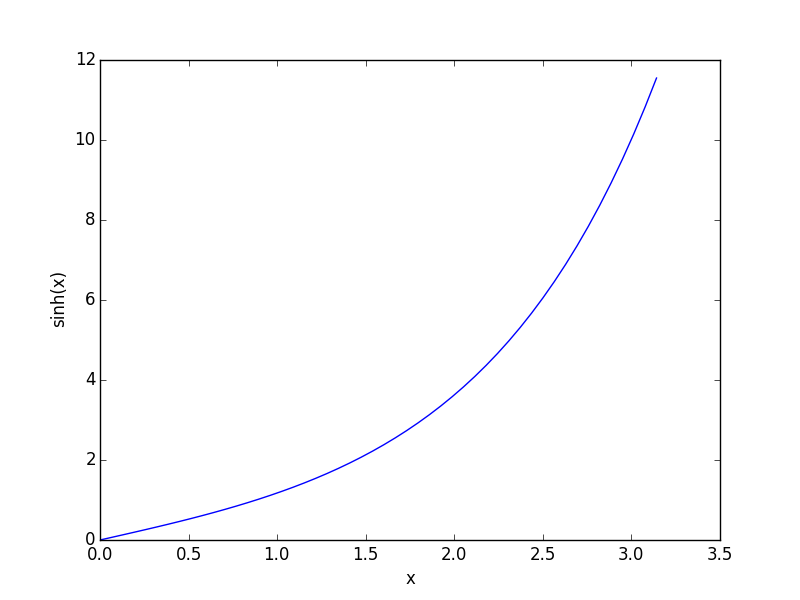
\includegraphics[width=.9\linewidth]{./sinh.png}
\caption{plotting is a cinch. \label{fig-cinch}}
\end{figure}

The results are in Figure \ref{fig-cinch}.

\section{Conclusions}
\label{sec:orgheadline4}
org-ref was used in these papers \cite{xu-2015-tunin-oxide,xu-2015-relat,xu-2015-linear-respon,xu-2015-accur-u,xu-2014-relat,xu-2014-probin-cover,miller-2014-simul-temper,mehta-2014-ident-poten,kitchin-2015-examp,kitchin-2015-data-surfac-scien,hallenbeck-2013-effec-o2,curnan-2014-effec-concen,boes-2015-estim-bulk-si,boes-2015-estim-bulk}.

It made it easy.

\bibliographystyle{unsrt}
\bibliography{/Users/jkitchin/Desktop/org-ref-example/manuscript,/Users/jkitchin/Dropbox/bibliography/references}
\end{document}
